\documentclass{article}
\usepackage{amsmath}
\usepackage{amsfonts}
\usepackage[english]{babel}
\usepackage[utf8]{inputenc}
\usepackage{amsthm}
\usepackage{graphicx}

\newcommand{\norm}[1]{\left\lVert#1\right\rVert}
\newtheorem{theorem}{Theorem}
\newtheorem{prop}{Proposition}
\newcommand{\overbar}[1]{\mkern 1.5mu\overline{\mkern-1.5mu#1\mkern-1.5mu}\mkern 1.5mu}

\begin{document}

\title{Mechanical Earth Hw2}
\author{Toby Harvey}
\maketitle
\noindent\textbf{Problem 1}

\noindent a) If $\theta = 120$ then, $ \vec{n} = \begin{bmatrix} \cos(120) \\ \sin(10)\\ \end{bmatrix} = \begin{bmatrix} -.5 \\ .866\\ \end{bmatrix}$, and the traction vector is then $$\vec{t}(\vec{n}) =
\begin{bmatrix}
  t_x\\
  t_y\\
\end{bmatrix}
= \begin{bmatrix}
  -40 && -60 \\
  -60 && -100 \\
\end{bmatrix}
\begin{bmatrix}
  -.5\\
  .866\\
\end{bmatrix}
=
\begin{bmatrix}
  -32 \text{ mN}\\
  -56 \text{ mN}\\
  \end{bmatrix}
$$

\vspace{3mm}

\noindent b) $|\vec{t}(\vec{n})| = \sqrt{(-32)^2 + (-56)^2} \approx 64 \text{ mN}$

\vspace{3mm}

\noindent $\alpha(\vec{n}) = \theta + \cos^{-1}\left(\frac{\vec{t}\cdot \vec{n}}{|\vec{t}||\vec{n}|}\right) = 120 + \cos^{-1}\frac{-.5(-32) + .866(-56)}{64 \cdot 1} = 120 + \cos^{-1}\left(-\frac{1}{2}\right) = 240^{\circ}$

\vspace{3mm}


\noindent d) We want to represent $\vec{t}(\vec{n})$  with respect to the normal and tangential  basis so just need to the transition matrix, since the normal is orthongal to the the tangential basis vector we:

\begin{gather*}
  \vec{n} \cdot \vec{s} = 0\\
  -.5(s_1) + .866(s_2) = 0\\
\end{gather*}

Picking an arbitrary $s_1 = 1$, then $s_2 = .5774$ and normilizing and accounting for the backwards orientation of the $s$ axis we get:

$$\vec{s} =
\begin{bmatrix}
  \frac{1}{\sqrt{1.\overbar{3}}}\\[4pt]
  -\frac{.5774}{\sqrt{1.\overbar{3}}}\\
\end{bmatrix}
  $$

so $\vec{t}(\vec{n})$ with respect to the normal tangential basis becomes:

$$\vec{t}^{\text{ }\prime}(\vec{n}) =
\begin{bmatrix}
  -.5 &&  \frac{1}{\sqrt{1.\overbar{3}}}\\[4pt]
  .866 && -\frac{.5774}{\sqrt{1.\overbar{3}}}\\
\end{bmatrix}
\begin{bmatrix}
  -32\\
  -56\\
\end{bmatrix}
=
\begin{bmatrix}
  -32.5 \text{ mN}\\
  55 \text{ mN}\\
\end{bmatrix}
  $$

Alternatively, we have:

\begin{gather*}
  t_n = t_x\cos\alpha + t_y\sin\alpha = -32(-.5) + -56(.866) = -32.5 \text{ mN}\\
  t_s = -t_x\sin\alpha + t_y\cos\alpha = -8.66(-32) + -.5(-56) = 55 \text{ mN}\\
\end{gather*}

Traction is consistent with shearing in figure one, since the positve shear axis is down to left, where this traction vector is pushing. It is also consistent with the normal vector in figure one, since the nomral is positive to the upper left, and the top slab is pushing downwards, meaning negative normal traction.

\vspace{3mm}

\noindent\textbf{Problem 2}

\noindent a) $\sigma_{\theta\theta}$ is maximized at $\theta = 0, 180$, because the second term is the largest there.

\noindent Setting $\sigma_{\theta\theta} = T$, and solving for P gives:

\begin{gather*}
  T = -\frac{1}{2}(S_H + S_h)\left[2\right]+ P + \frac{1}{2}(S_H - s_h)\left[ 4\right]\\
  \implies P\left(\frac{R}{r}\right)^2 = T + \frac{1}{2}(S_H + S_h)\left[ 2\right] -  \frac{1}{2}(S_H - s_h)\left[4\right]\\
  \implies P = \frac{r^2}{R^2} \left(T + \frac{1}{2}(S_H + S_h)\left[ 2\right] -  \frac{1}{2}(S_H - s_h)\left[ 4\right]\right)\\
  \implies P =  \left(T + (S_H + S_h) -  2(S_H - S_h)\right)\\
  \implies P =  T + S_H + s_h -2S_H + 2S_h\\
  \implies P = T - S_H + 3S_h
\end{gather*}


\vspace{3mm}

\noindent b) Looking at Figure 2, $R$ looks like it is about 3 km, and stress is greatest / the dike will initate at $r = R$, so for Tensile strength of 1 and 10 mPa:

\begin{gather*}
  P = 1 - 125 + 300 = 176 \text{ mPa}\\
  P = 10 -125 + 300 = 185 \text{ mPa}\\
\end{gather*}
 
\noindent If we model the pressure in the magma chamber as the lithostatic pressure at $d=4000\text{ m}$ then  we get that:

$$P = g\rho d = 9.8(4000)(2500) = 9.8\times10^7 \text{ Pa} = 98 \text{ mPa}$$

and therefore the magma pressure would not cause the rock to fracture.


\vspace{3mm}

\noindent c) In the matlab code, as $S_h$ approaches $S_H$, and visa versa, we see that the most compressive force moves towards the y axis, meaning that once $S_h$ surpasses $S_H$ then the magma chamber will fracture vertically. Notationally this is a little  bit confusing, because if $S_h$ becomes greater than $S_H$ then $S_h$ really is suppose to become $S_H$.

At future distances from the magma chamber we can figure out what $S_H$ and $s_h$ are, because the dike will form in the direction of the most compressive stress or $S_H$, and we know it will have ``opened'' in that direction of least stress $S_h$, because the local conditions of the magma chamber become negligable.

If the dikes are purely radial, we know that $S_H \approx S_h$, because the direction the dike is facing hasn't changed the further we move from the magma chamber.

\noindent\textbf{Problem 3}

Here is the output from my matlab code:

\vspace{3mm}

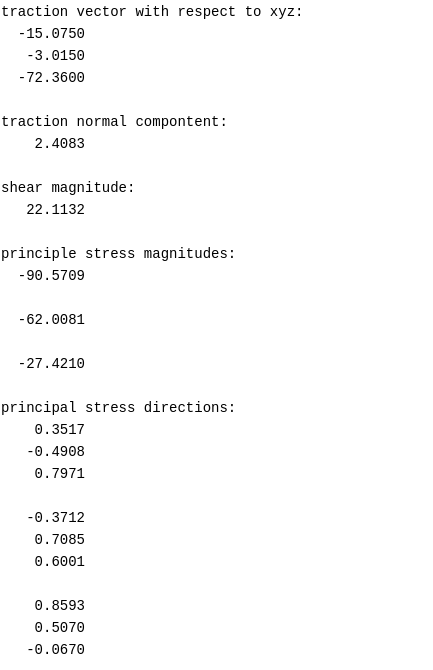
\includegraphics[scale=.5]{output.png}


Which would mean that: $$\sigma_1 =
\begin{bmatrix}
  .86\\
  .50\\
  .06\\
\end{bmatrix}
\qquad
\sigma_2 =
\begin{bmatrix}
  -.37\\
  .71\\
  .60\\
\end{bmatrix}
$$
\end{document}
